\chapter{RESULTADOS}\label{chap:resuldatos}

A seguir são apresentados os resultados obtidos \ldots

\section{Secao 1}\label{sec:Secao_1}
Na figura~\ref{fig:figura50}\ldots

\begin{figure}[H]
    \centering
    \caption{Testes 1}
    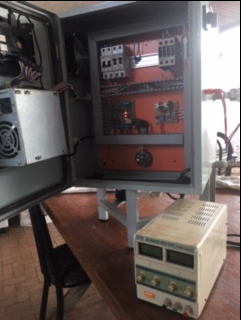
\includegraphics[width=0.6\textwidth]{figuras/figu50.png}
    \fonte{Algum lugar sujo}
    \label{fig:figura50}
\end{figure}

\section{Secao 2}\label{sec:Secao_2}

Na figura~\ref{fig:figura44}, foi realizado \ldots

\begin{figure}[H]
    \centering
    \caption{Testes 2}\label{fig:figura44}
    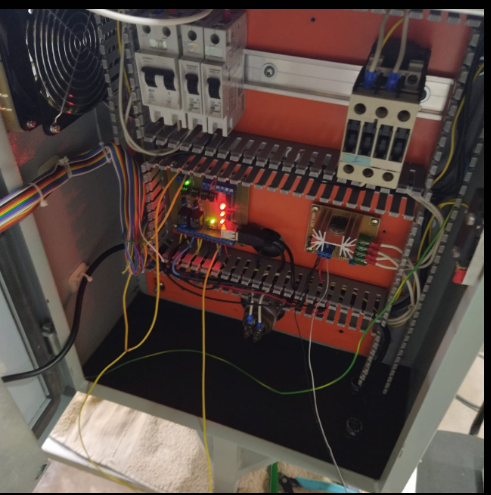
\includegraphics[width=0.6\textwidth]{figuras/figu44.png}
    \fonte{O mesmo lugar sujo}
\end{figure}

Não foi possível realizar e finalizar todos os testes como: \ldots devido a pandemia do $COVI19$ de acordo com o DECRETO No 64.864, no dia 16 de março de 2020,onde as atividades em sala de aula, que eram presenciais, ficaram suspensas, e também teve início o distanciamento social
